\section{Bevægelsesanalyse}
%Indhold:
%- Hvad er bevægelse
%	- definition og opståen 
%- Hvordan måles bevægelse
%- Karakteristika for forskellige bevægelser 
%	- Sammenligning af de forskellige aktiviteter
%		- hvordan adskiller de sig fra hinanden
%
\textit{Følgende afsnit indeholder bevægelsesanalyser for gang, løb og cykling. Dette medhenblik på at finde karakteristika for de tre aktiviteter, hvorledes deres forskelle senere vil kunne være behjælpelige i forbindelse med detektering af de enkelte aktiviteter. Der vil derfor afslutningsvist være en sammenligning af karakteristika for de tre aktiviteter}

\subsection{Gang}
Gang er en fysisk aktivitet kendetegnet ved altid at have et ben på jorden. Aktiviteten betegnes som en cyklus, da den samme række bevægelser gentages for at udføre aktiviteten. Bevægelserne er desuden identiske for højre og venstre ben, men forskudt med en halv cyklus, hvorfor bevægelsen kun vil blive beskrevet for højre ben. \citep{VaughanDavisOConnor1992,Whittle1990} 

En gangcyklus inddeles i to faser, standfasen og svingfasen, hvilket fremgår af \figref{fig:gang_cyklus}. Standfasen har en varighed svarende til cirka 60\% af en gangcyklus, og påbegyndes idet den højre fod opnår kontakt med underlaget. Fasen indebærer den tid hvor højre fod er i berøring med jorden. Svingfasen udgør derimod cirka 30\% af hele gangcyklussen, og er den periode, hvor foden og benet bevæges frem og derfor ikke er i berøring med jorden. Efter denne fase, er foden igen klar til isætning af højre hæl. \citep{VaughanDavisOConnor1992}

\begin{figure}[H]
	\centering
	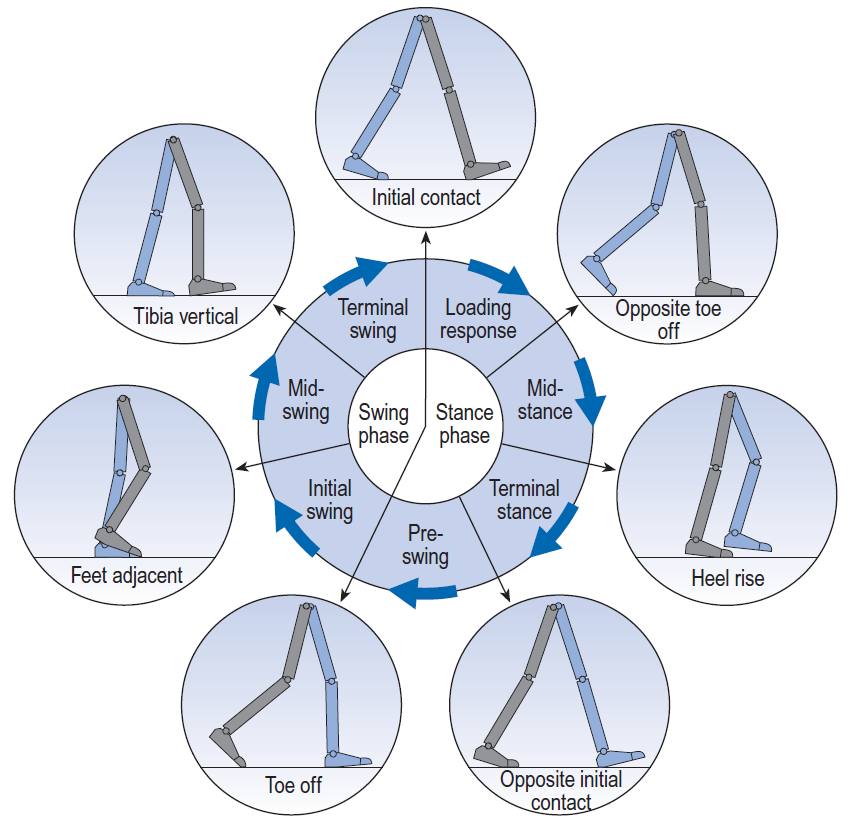
\includegraphics[scale=0.5]{figures/bProblemloesning/gang_cyklus2.png}
	\caption{På figuren ses en gangcyklus opdelt i standfase og svingfase. \citep{VaughanDavisOConnor1992}}
	\label{fig:gang_cyklus}
\end{figure}
\fxnote{SKAL MODIFICERES. Gør så at figuren også har den procentvise fordeling af faserne på +++ DET ER DEN FORKERTE KILDE SOM ER SAT PÅ?}
	
Som det fremgår af billedet, er standfasen og svingfasen yderligere inddelt henholdsvis i 5 og 3 faser. \newline
Standfasens første fase er et hæl-nedslag, som starter hele cyklussen, hvilket opnås når den højre hæl kommer i kontakt med jordoverfladen. Herefter er foden flad og den venstre fod er derimod i berøring med overfladen med tåspidserne. Hælen på den højre fod løftes nu, alt i mens den venstre fod, som er i svingfasen, passerer den højre fod. Der opstår nu et hæl-slip for den højre fod, og der skabes en berøring af den venstre fod på underlaget. Standfasen afsluttes med en fleksion af anklen og dermed et afsæt fra tæerne på højre fod. \newline
Den højre fod, og det højre ben, er dermed i svingfasen, som påbegyndes med en acceleration af foden og benet. Denne acceleration begynder når foden ikke længere har kontakt med underlaget i standfasen. Derfor vil det højre ben blive bevæget frem mod det venstre ben. Efterfølgende vil der være et såkaldt, midt-sving som forekommer når højre fod er lige under kroppen og dermed ud for den venstre fod, som er i kontatkt med jorden. Afsluttende for svingfasen er der en deacceleration. Denne fase involverer en række muskler som sænker hastigheden af benet og fodens fremadgående bevægelse, således kroppen er klar til det kommende hæl-nedslag i standfasen.


\subsection{Løb}
Løb er en aktivitet karakteriseret ved, at kun én fod rør jorden ad gangen. Denne aktivitet beskrives, ligesom gang, som en cyklus der gennemgår forskellige faser. Denne aktivitet karakteriseres som en hurtigere variation af gang, hvor kun én fod rør jorden ad gangen. Løbecyklussen består derfor af fire faser, som vist på \figref{fig:loebecyklus}: standfasen, den første svævefase, svingfasen og den anden svævefase. \citep{Adelaar1986,Novacheck1998}

\begin{figure}[H]
	\centering
	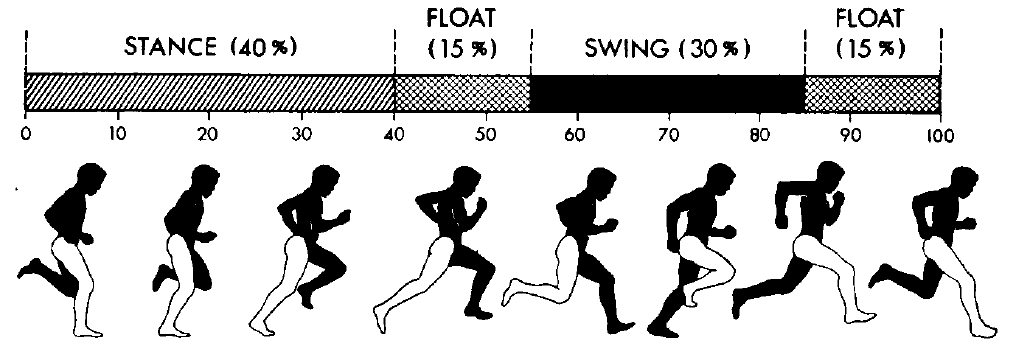
\includegraphics[scale=0.4]{figures/bProblemloesning/loeb_cyklus1.png}
	\caption{På figuren ses en løbecyklus opdelt i standfase, svingfase og to svævefaser. \citep{Adelaar1986}}
	\label{fig:loebecyklus}
\end{figure}
\fxnote{SKAL MODIFICERES}

På samme vis som ved gangcyklussen, initieres løbecyklussen idet den højre hæl rammer jorden, hvilket er begyndelsen af den første fase, standfasen, som udgør 40\% af løbecyklussen. Herefter fortsætter foden til midt stand, og afslutningsvis afsættes der med tæerne, hvilket leder op til den næste fase, den første svævefase. De to svævefaser, som går igen to gange i løbecyklussen, er identiske og udgør hver 15\% af cyklussen. Disse er karakteriseret ved at begge ben er løftet fra jorden. Mellem de to svævefaser, er svingfasen, som udgør 30\%. Denne fase initieres idet hælen hæves og knæet føres frem, hvorefter hælen igen sænkes\fxnote{i denne fase er den modsatte fod i jorden}, og svævefasen gentages, før en ny cyklus kan påbegyndes. \citep{Adelaar1986,Novacheck1998}

\fxnote{Længden af disse faser varierer dog alt efter hvor hurtigt man løber, da svævefasen øges.} 

Løb er karakteriseret ved, at kun én fod rør jorden ad gangen. Dette resulterer i at der er et større stress på leddene ved løb i forhold til gang. Eksempelvis vil en person på 68 kg have et stress på sin fod på 35 kg/m ved gang, mens det ved løb vil være et stress på 110 ton/m.\fxnote{KILDE - JOSE}

\fxnote{Tjek bog om der er mere eller om det muligvis er en bedre/nyere kilde}













